%! Mode:: "TeX:UTF-8"
%! TEX program = xelatex
\PassOptionsToPackage{quiet}{xeCJK}
\documentclass[withoutpreface,notoc]{cumcmthesis}

\usepackage[super,numbers,sort&compress]{natbib}
\usepackage[framemethod=TikZ]{mdframed}
\usepackage{pdfpages}
\usepackage{etoolbox}
\BeforeBeginEnvironment{tabular}{\zihao{-5}}
\newcolumntype{C}{>{\centering\arraybackslash}X}
\newcolumntype{R}{>{\raggedleft\arraybackslash}X}
\newcolumntype{L}{>{\raggedright\arraybackslash}X}
\lstset{
  language=Python,
  basicstyle=\ttfamily\zihao{6},
  numbers=left,
  numberstyle=\tiny,
  stepnumber=1,
  numbersep=8pt,
  frame=single,
  breaklines=true,
  columns=fullflexible,
  keepspaces=true,
  showstringspaces=false,
  tabsize=4,
  captionpos=b
}

\title{基于几何覆盖与分区智能优化的多波束测线设计}

\begin{document}
\maketitle

\begin{abstract}
多波束测深的核心是在复杂海底地形下协调覆盖完整性、条带重叠率与航行总里程。本文从声束与倾斜海底的几何交会关系出发，建立由二维斜坡推广到三维海底平面的覆盖宽度模型，并进一步构造矩形海域和真实离散地形上的测线优化模型。

\textbf{针对问题一，}在垂直测线的剖面内建立左右边缘波束与倾斜海底的几何模型，区分斜面实际覆盖宽度与水平投影覆盖宽度，并以相邻测线相向半宽计算重叠率。结果表明，当测线由深水侧移向浅水侧时，水深由 $90.95\,\mathrm m$ 降至 $49.05\,\mathrm m$，水平投影覆盖宽度由 $315.71\,\mathrm m$ 降至 $170.27\,\mathrm m$；固定 $200\,\mathrm m$ 间距会使浅水端出现漏测。

\textbf{针对问题二，}建立海底平面模型，通过测线方向角 $\beta$ 将真实坡度转化为横向扫描剖面内的等效坡度 $\alpha_\beta$，得到任意船位和方向下的覆盖宽度。计算显示，沿等深线方向航行时横向剖面坡度最大，而沿最大坡降方向航行时横向剖面近似水平；所得 $8\times8$ 覆盖宽度表满足题目要求。

\textbf{针对问题三，}以测线方向、截距及目标重叠率为决策变量，以总测量长度最短为目标，建立带完全覆盖及 $10\%\sim20\%$ 重叠约束的优化模型。采用粗网格角度搜索与黄金分割精修，并以改进粒子群算法复核。最优方向角为 $90^\circ$，共布设 34 条南北向测线，总长度为 $68.000$ 海里，重叠率稳定在 $10\%$。

\textbf{针对问题四，}先由题目提供的离散测深数据构造连续等深线场，再对标准化后的东西坐标、南北坐标和水深进行加权 K-means 聚类，结合簇内平方和与分区可解释性取 $K=4$。在各分区内沿等深线生成曲线测线，并利用粒子群优化各区目标重叠率。最终方案包含 86 条曲线，总长度为 $210.650322$ 海里。程序在分区深度带递推模型内得到漏测标志与超额重叠等效长度均为 0；其中漏测标志尚未经过独立二维网格面积复核，故不将其解释为实际航测中的严格零漏测。

在直线声传播、缓变坡面和离散分区等假设下，模型具有明确的物理意义和可复现的计算流程，可为不规则测区的多波束测线规划提供一种候选框架。

\keywords{多波束测深\quad 覆盖宽度\quad 重叠率\quad K-means聚类\quad 粒子群优化}
\end{abstract}

\section{问题重述}
多波束测深系统在测量船航迹两侧形成条带。条带宽度随换能器开角、水深、海底坡度和测线方向变化。根据赛题原文\cite{cumcm2023b}，题目要求：第一，建立倾斜海底上覆盖宽度及相邻条带重叠率模型并完成表1；第二，将模型推广到测线方向任意的三维情形并完成表2；第三，在 $4$ 海里乘 $2$ 海里的理想斜坡海域内设计完全覆盖、重叠率为 $10\%\sim20\%$ 且总长度最短的测线；第四，利用附件的真实测深数据设计测线，并计算总长度、漏测率和超额重叠长度。

四个问题由局部覆盖几何逐层递进到全局路径优化。问题一、二提供任意位置的覆盖宽度函数，问题三、四则以该函数为基础决定测线方向、位置和间距。

\section{问题分析}
倾斜海底上左右两侧声束的作用距离不对称，因此不能直接套用平底公式 $W=2D\tan(\theta/2)$。此外，测线间距在水平面内度量，而波束交点间距离沿斜坡度量，两者必须投影到同一平面。问题二的关键是求测线横向剖面的等效坡度。问题三是在连续方向空间中求最短平行测线组；问题四地形非平面，应先将地形分区，再以等深线作为局部测线方向，使测线尽可能沿同一水深行驶，从而稳定覆盖宽度。

\section{模型假设}
\begin{itemize}[itemindent=2em]
  \item 声波在海水中沿直线传播，忽略声速剖面、海面起伏及折射；该处理是理想化几何近似，真实水声传播会受到介质声速结构影响\cite{lurton}。
  \item 换能器边缘波束关于铅垂方向对称，开角恒定为 $120^\circ$。
  \item 问题一至三的海底为理想平面；局部范围内坡度连续。
  \item 船体姿态和定位误差相对测区尺度较小，暂不计入覆盖边界。
  \item 附件测深数据可靠；网格插值得到的地形可代表测量时海底地形。
  \item 问题四以离散网格单元统计覆盖与漏测，曲线长度由等深线折线段累加。
\end{itemize}

\section{符号说明}
\begin{table}[H]
\centering
\caption{主要符号说明}
\label{tab:symbols}
\begin{tabularx}{\textwidth}{CLC}
\toprule
符号 & 含义 & 单位\\
\midrule
$\theta,\gamma$ & 换能器开角与半开角，$\gamma=\theta/2$ & $^\circ$\\
$\alpha$ & 海底最大坡度 & $^\circ$\\
$\beta$ & 测线方向与坡面法向水平投影的夹角 & $^\circ$\\
$D,D_0$ & 船位水深与中心水深 & m\\
$W_s,W_h$ & 斜面实际覆盖宽度与水平投影宽度 & m\\
$L_l,L_r$ & 左、右侧水平投影覆盖半宽 & m\\
$d$ & 相邻测线水平间距 & m\\
$\eta$ & 相邻条带重叠率 & \%\\
$\varphi$ & 平面内测线方向角 & $^\circ$\\
$N,L$ & 测线数与测线总长度 & 条、海里\\
\bottomrule
\end{tabularx}
\end{table}
为统一角度单位，本文所有角度的输入、表格与结果均以度表示。若 $a$ 为以度表示的角度，则下文公式中的 $\sin a$、$\cos a$ 和 $\tan a$ 分别约定为
$\sin(\pi a/180)$、$\cos(\pi a/180)$ 和 $\tan(\pi a/180)$；程序内部亦先转换为弧度再调用三角函数。

\section{问题一：倾斜剖面的覆盖与重叠模型}
\subsection{水深与覆盖宽度}
以海域中心为原点，令 $x$ 轴正向指向浅水侧，则
\begin{equation}\label{eq:depth1}
D(x)=D_0-x\tan\alpha.
\end{equation}
在垂直测线的剖面内，由正弦定理，边缘波束在海底斜面上的左右覆盖半宽为
\begin{equation}\label{eq:sideslope}
L^s_l(x)=\frac{D(x)\sin\gamma}{\cos(\gamma+\alpha)},\qquad
L^s_r(x)=\frac{D(x)\sin\gamma}{\cos(\gamma-\alpha)}.
\end{equation}
故斜面实际覆盖宽度与水平投影宽度分别为
\begin{align}
W_s(x)&=D(x)\sin\gamma\left[\frac1{\cos(\gamma+\alpha)}+\frac1{\cos(\gamma-\alpha)}\right],\label{eq:ws}\\
W_h(x)&=W_s(x)\cos\alpha.\label{eq:wh}
\end{align}
当 $\alpha=0$ 时，上式退化为 $W_s=W_h=2D\tan\gamma$，与平坦海底公式一致。

\subsection{相邻条带重叠率}
水平面上的左右半宽为 $L_l=L_l^s\cos\alpha$、$L_r=L_r^s\cos\alpha$。测线按 $x$ 递增排列，$d=x_i-x_{i-1}$，则相邻条带的交叠长度为
\begin{equation}
\Delta_i=L_r(x_{i-1})+L_l(x_i)-d.
\end{equation}
以第 $i$ 条测线覆盖宽度归一化，得到
\begin{equation}\label{eq:eta}
\eta_i=\frac{L_r(x_{i-1})+L_l(x_i)-d}{W_h(x_i)}\times100\%.
\end{equation}
$\eta_i<0$ 表示存在空隙，即发生漏测。

\subsection{计算结果}
代入 $\theta=120^\circ$、$\alpha=1.5^\circ$、$D_0=70\,\mathrm m$、$d=200\,\mathrm m$，结果见\cref{tab:q1}。
\begin{table}[H]
\centering
\caption{问题一计算结果}
\label{tab:q1}
\resizebox{\textwidth}{!}{
\begin{tabular}{c|rrrrrrrrr}
\toprule
距中心距离/m&$-800$&$-600$&$-400$&$-200$&0&200&400&600&800\\
\midrule
海水深度/m&90.95&85.71&80.47&75.24&70.00&64.76&59.53&54.29&49.05\\
覆盖宽度/m&315.71&297.53&279.35&261.17&242.99&224.81&206.63&188.45&170.27\\
与前一条重叠率/\%&--&35.70&31.51&26.74&21.26&14.89&7.41&$-1.53$&$-12.36$\\
\bottomrule
\end{tabular}}
\end{table}
固定间距下，浅水侧覆盖宽度快速缩小，$x=600\,\mathrm m$ 后出现漏测。说明实际布线必须随水深动态缩小测线间距。

\begin{figure}[H]
\centering
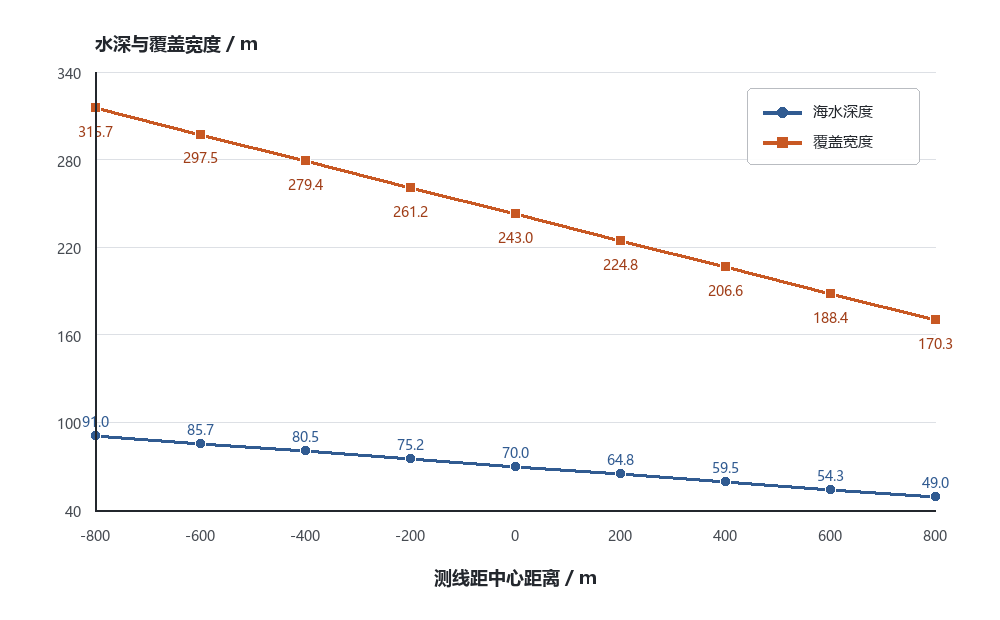
\includegraphics[width=0.94\textwidth]{问题一/paper_q1_revised_20260713.png}
\caption{问题一水深与覆盖宽度变化}
\label{fig:q2}
\end{figure}

\section{问题二：任意测线方向的三维覆盖模型}
\subsection{海底平面与等效坡度}
令 $x$ 轴沿最大坡降的反方向（浅水方向），$y$ 轴沿等深线，则
\begin{equation}
D(x,y)=D_0-x\tan\alpha.
\end{equation}
测线方向单位向量和其水平法向量分别为
\begin{equation}
\boldsymbol e_l=(\cos\beta,\sin\beta),\qquad
\boldsymbol e_p=(-\sin\beta,\cos\beta).
\end{equation}
船距中心 $s$ 时，取船位为 $s\boldsymbol e_l$，船位水深为
\begin{equation}\label{eq:depth2}
D_s=D_0-1852s\cos\beta\tan\alpha,
\end{equation}
其中 $s$ 以海里计。沿横向扫描方向移动 $u$，水深变化率为 $\mathrm dD/\mathrm du=\sin\beta\tan\alpha$，故等效坡度满足
\begin{equation}\label{eq:alphab}
\alpha_\beta=\arctan(\sin\beta\tan\alpha).
\end{equation}
将问题一中的 $D(x),\alpha$ 分别替换为 $D_s,\alpha_\beta$，得到
\begin{equation}\label{eq:q2width}
W_s(s,\beta)=D_s\sin\gamma\left[\frac1{\cos(\gamma+\alpha_\beta)}+\frac1{\cos(\gamma-\alpha_\beta)}\right].
\end{equation}

\subsection{计算结果}
代入中心水深 $120\,\mathrm m$，得到题目所需斜面实际覆盖宽度，见\cref{tab:q2}。
\begin{table}[H]
\centering
\caption{问题二覆盖宽度（m）}
\label{tab:q2}
\resizebox{\textwidth}{!}{
\begin{tabular}{c|rrrrrrrr}
\toprule
$\beta/{}^\circ\backslash s$/海里&0&0.3&0.6&0.9&1.2&1.5&1.8&2.1\\
\midrule
0&415.69&365.29&314.89&264.50&214.10&163.70&113.30&62.90\\
45&416.19&380.51&344.83&309.15&273.47&237.79&202.11&166.43\\
90&416.69&416.69&416.69&416.69&416.69&416.69&416.69&416.69\\
135&416.19&451.87&487.55&523.23&558.91&594.59&630.27&665.95\\
180&415.69&466.09&516.49&566.89&617.29&667.69&718.09&768.48\\
225&416.19&451.87&487.55&523.23&558.91&594.59&630.27&665.95\\
270&416.69&416.69&416.69&416.69&416.69&416.69&416.69&416.69\\
315&416.19&380.51&344.83&309.15&273.47&237.79&202.11&166.43\\
\bottomrule
\end{tabular}}
\end{table}
当 $\beta=0^\circ,180^\circ$ 时横向剖面沿等深线，$\alpha_\beta=0$；当 $\beta=90^\circ,270^\circ$ 时横向剖面沿最大坡度方向，$|\alpha_\beta|=\alpha$。这些退化情形验证了模型的合理性。
由\cref{tab:q2}还可看出明显的方向性：$\beta=90^\circ$ 和 $270^\circ$ 时，船位沿等深线移动，所在水深保持不变，因此各距离上的覆盖宽度均为 $416.69\,\mathrm m$；$\beta=0^\circ$ 时船向浅水侧移动，覆盖宽度由 $415.69\,\mathrm m$ 单调减至 $62.90\,\mathrm m$；$\beta=180^\circ$ 时船向深水侧移动，覆盖宽度增至 $768.48\,\mathrm m$。其余方向介于上述典型情形之间，并关于 $180^\circ$ 方向呈对称变化。表格直接给出了全部数值，较色块图更便于复核和引用。

\section{问题三：理想矩形海域的最短测线设计}
\subsection{优化模型}
将海区换算为 $[-2,2]\times[-1,1]$ 海里。设测线方向为 $\varphi$，沿线单位向量为 $\boldsymbol u=(\cos\varphi,\sin\varphi)$，法向量为 $\boldsymbol n=(-\sin\varphi,\cos\varphi)$，第 $i$ 条测线写为
\begin{equation}
\boldsymbol n\cdot\boldsymbol p=r_i.
\end{equation}
测线与矩形边界相交所得线段长度记为 $l_i$。目标函数为
\begin{equation}\label{eq:q3obj}
\min_{\varphi,\{r_i\},N} L=\sum_{i=1}^{N}l_i,
\end{equation}
约束为所有测线覆盖条带的并集包含整个矩形，且相邻条带满足
\begin{equation}
0.10\leq \frac{b_i^R+b_{i+1}^L-(r_{i+1}-r_i)}{\min(W_i,W_{i+1})}\leq0.20.
\end{equation}
其中 $b_i^L,b_i^R$ 由\cref{eq:sideslope}投影得到。为使总长度最短，在给定方向下取约束允许的最小重叠率 $10\%$，从深水边界开始递推各测线位置。

\subsection{求解算法}
先在方向角区间内以 $0.1^\circ$ 步长粗搜索，对每个方向用二分法求首条测线和后续测线截距；再在粗搜索最优角附近用黄金分割法精修。另构造改进粒子群算法\cite{pso}，以 $\varphi$、方向渐变量和目标重叠率为粒子位置。

为说明罚项，记测区在测线法向上的投影边界为 $r_{\min},r_{\max}$，第 $i$ 条覆盖带的左右边界坐标为 $c_i^L,c_i^R$。定义深水端和浅水端未覆盖宽度
\[
P_{\rm miss}^{d}=\frac{\max(0,r_{\max}-c_1^R)}{1852},\qquad
P_{\rm miss}^{s}=\frac{\max(0,c_N^L-r_{\min})}{1852},
\]
并定义第 $i$ 对相邻测线的重叠违规量
\[
P_{\eta,i}=\max\{0,\ 0.10-\eta_i,\ \eta_i-0.20\}.
\]
三者分别衡量两端漏测和重叠率越界，均在可行解上取 0。适应度为总长度与上述罚项之和：
\begin{equation}
F=\frac{L}{1852}+10^6(P_{\rm miss}^{d}+P_{\rm miss}^{s})+10^5\sum_i P_{\eta,i}^2.
\end{equation}
两种算法均收敛到 $\varphi=90^\circ$，说明测线沿南北短边布设最优：每条长 2 海里，同时测线法向与水深变化方向一致，能够按局部水深调整间距。

\subsection{结果分析}
最终共 34 条测线，每条长度为 2 海里，总长 $68.000$ 海里。最西侧测线位于 $x=-3345.48\,\mathrm m$，最东侧位于 $x=3697.57\,\mathrm m$；未舍入结果的相邻重叠率最小值与最大值均为 $10.000\%$，导出的两位小数边界数据复算范围为 $9.990\%\sim10.009\%$。首条覆盖带到达东边界 $x=3704.00\,\mathrm m$，末条覆盖带左边界为 $x=-3719.41\,\mathrm m<-3704\,\mathrm m$，故横向边界被覆盖。随着水深减小，覆盖宽度由 $685.93\,\mathrm m$ 减至 $45.74\,\mathrm m$，测线间距随之递减。

\cref{fig:q3}以由深到浅的连续底色表示西深东浅的水深梯度，白色竖线为实际南北向测线，线中编号用于标识测线顺序，橙色窄带表示相邻条带的重叠区域。图中西侧测线较疏、东侧测线显著加密，直观反映覆盖宽度随水深变浅而缩小；测线贯穿南北边界，说明纵向不存在漏测。原图摘要中的最优方向角 $90^\circ$、34 条测线、总长 68 海里及约 $10\%$ 的重叠率均已在本段集中说明。

\begin{figure}[H]
\centering
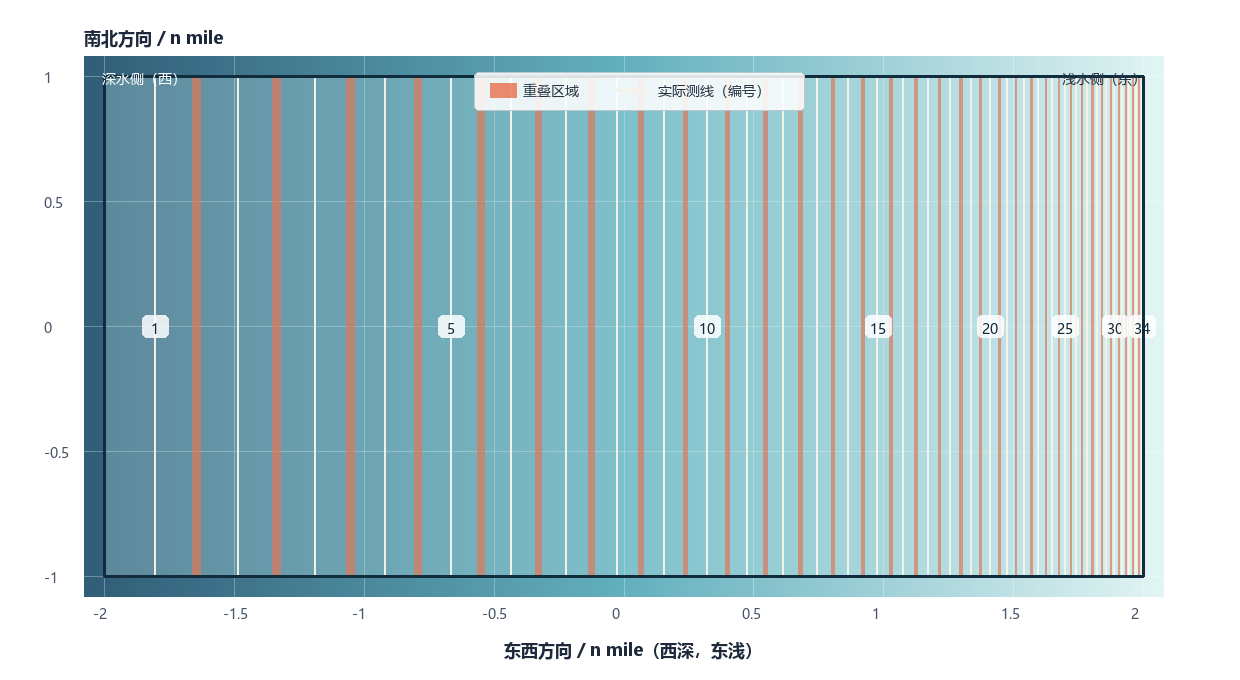
\includegraphics[width=0.96\textwidth]{问题三/paper_q3_revised_20260713.png}
\caption{问题三最优测线布设}
\label{fig:q3}
\end{figure}

\section{问题四：真实地形的分区曲线测线设计}
\subsection{地形重建与空间--水深聚类}
读取附件中东西坐标、南北坐标与水深矩阵，形成测深点集 $\{(x_j,y_j,z_j)\}$，通过规则网格插值和等深线提取得到连续地形。为兼顾空间连通性和深度相似性，对三维特征分别标准化，并提高水深权重：
\begin{equation}
\boldsymbol q_j=\left(\frac{x_j-\bar x}{s_x},\frac{y_j-\bar y}{s_y},1.6\frac{z_j-\bar z}{s_z}\right).
\end{equation}
K-means\cite{kmeans,lloyd} 的目标为
\begin{equation}
\min\sum_{k=1}^{K}\sum_{\boldsymbol q_j\in C_k}\|\boldsymbol q_j-\boldsymbol\mu_k\|_2^2.
\end{equation}
计算 $K=2,\ldots,10$ 的簇内平方和。前五个候选值见\cref{tab:kmeans-elbow}；$K$ 从 2 增至 4 时平方和明显下降，而继续增加 $K$ 会提高分区与测线衔接复杂度，因此将 $K=4$ 作为精度与可解释性的折中选择，而非声称其为唯一最优分区数。
\begin{table}[H]
\centering
\caption{K-means 分区数选择依据}
\label{tab:kmeans-elbow}
\begin{tabular}{c|rrrrr}
\toprule
$K$ & 2 & 3 & 4 & 5 & 6\\
\midrule
簇内平方和 & 126377.4 & 74588.9 & 56415.2 & 44935.6 & 35906.4\\
\bottomrule
\end{tabular}
\end{table}

附件共形成 50451 个有效测深网格点，水深范围为 $20.00\sim197.20\,\mathrm m$，等深线间隔取 $10\,\mathrm m$。\cref{fig:q4a}表明西南部整体较浅、东南角水深快速增加，北部水深变化相对平缓。空间--水深聚类得到四个区域：区域1水深 $20.0\sim64.1\,\mathrm m$，占 $33.9\%$；区域2为 $42.7\sim84.8\,\mathrm m$，占 $23.8\%$；区域3为 $50.4\sim102.1\,\mathrm m$，占 $31.6\%$；区域4为 $88.5\sim197.2\,\mathrm m$，占 $10.8\%$。由于聚类同时考虑空间位置，区域间水深范围允许交叠，这并不表示分类冲突。

\begin{figure}[H]
\centering
\subcaptionbox{附件地形等深线\label{fig:q4a}}{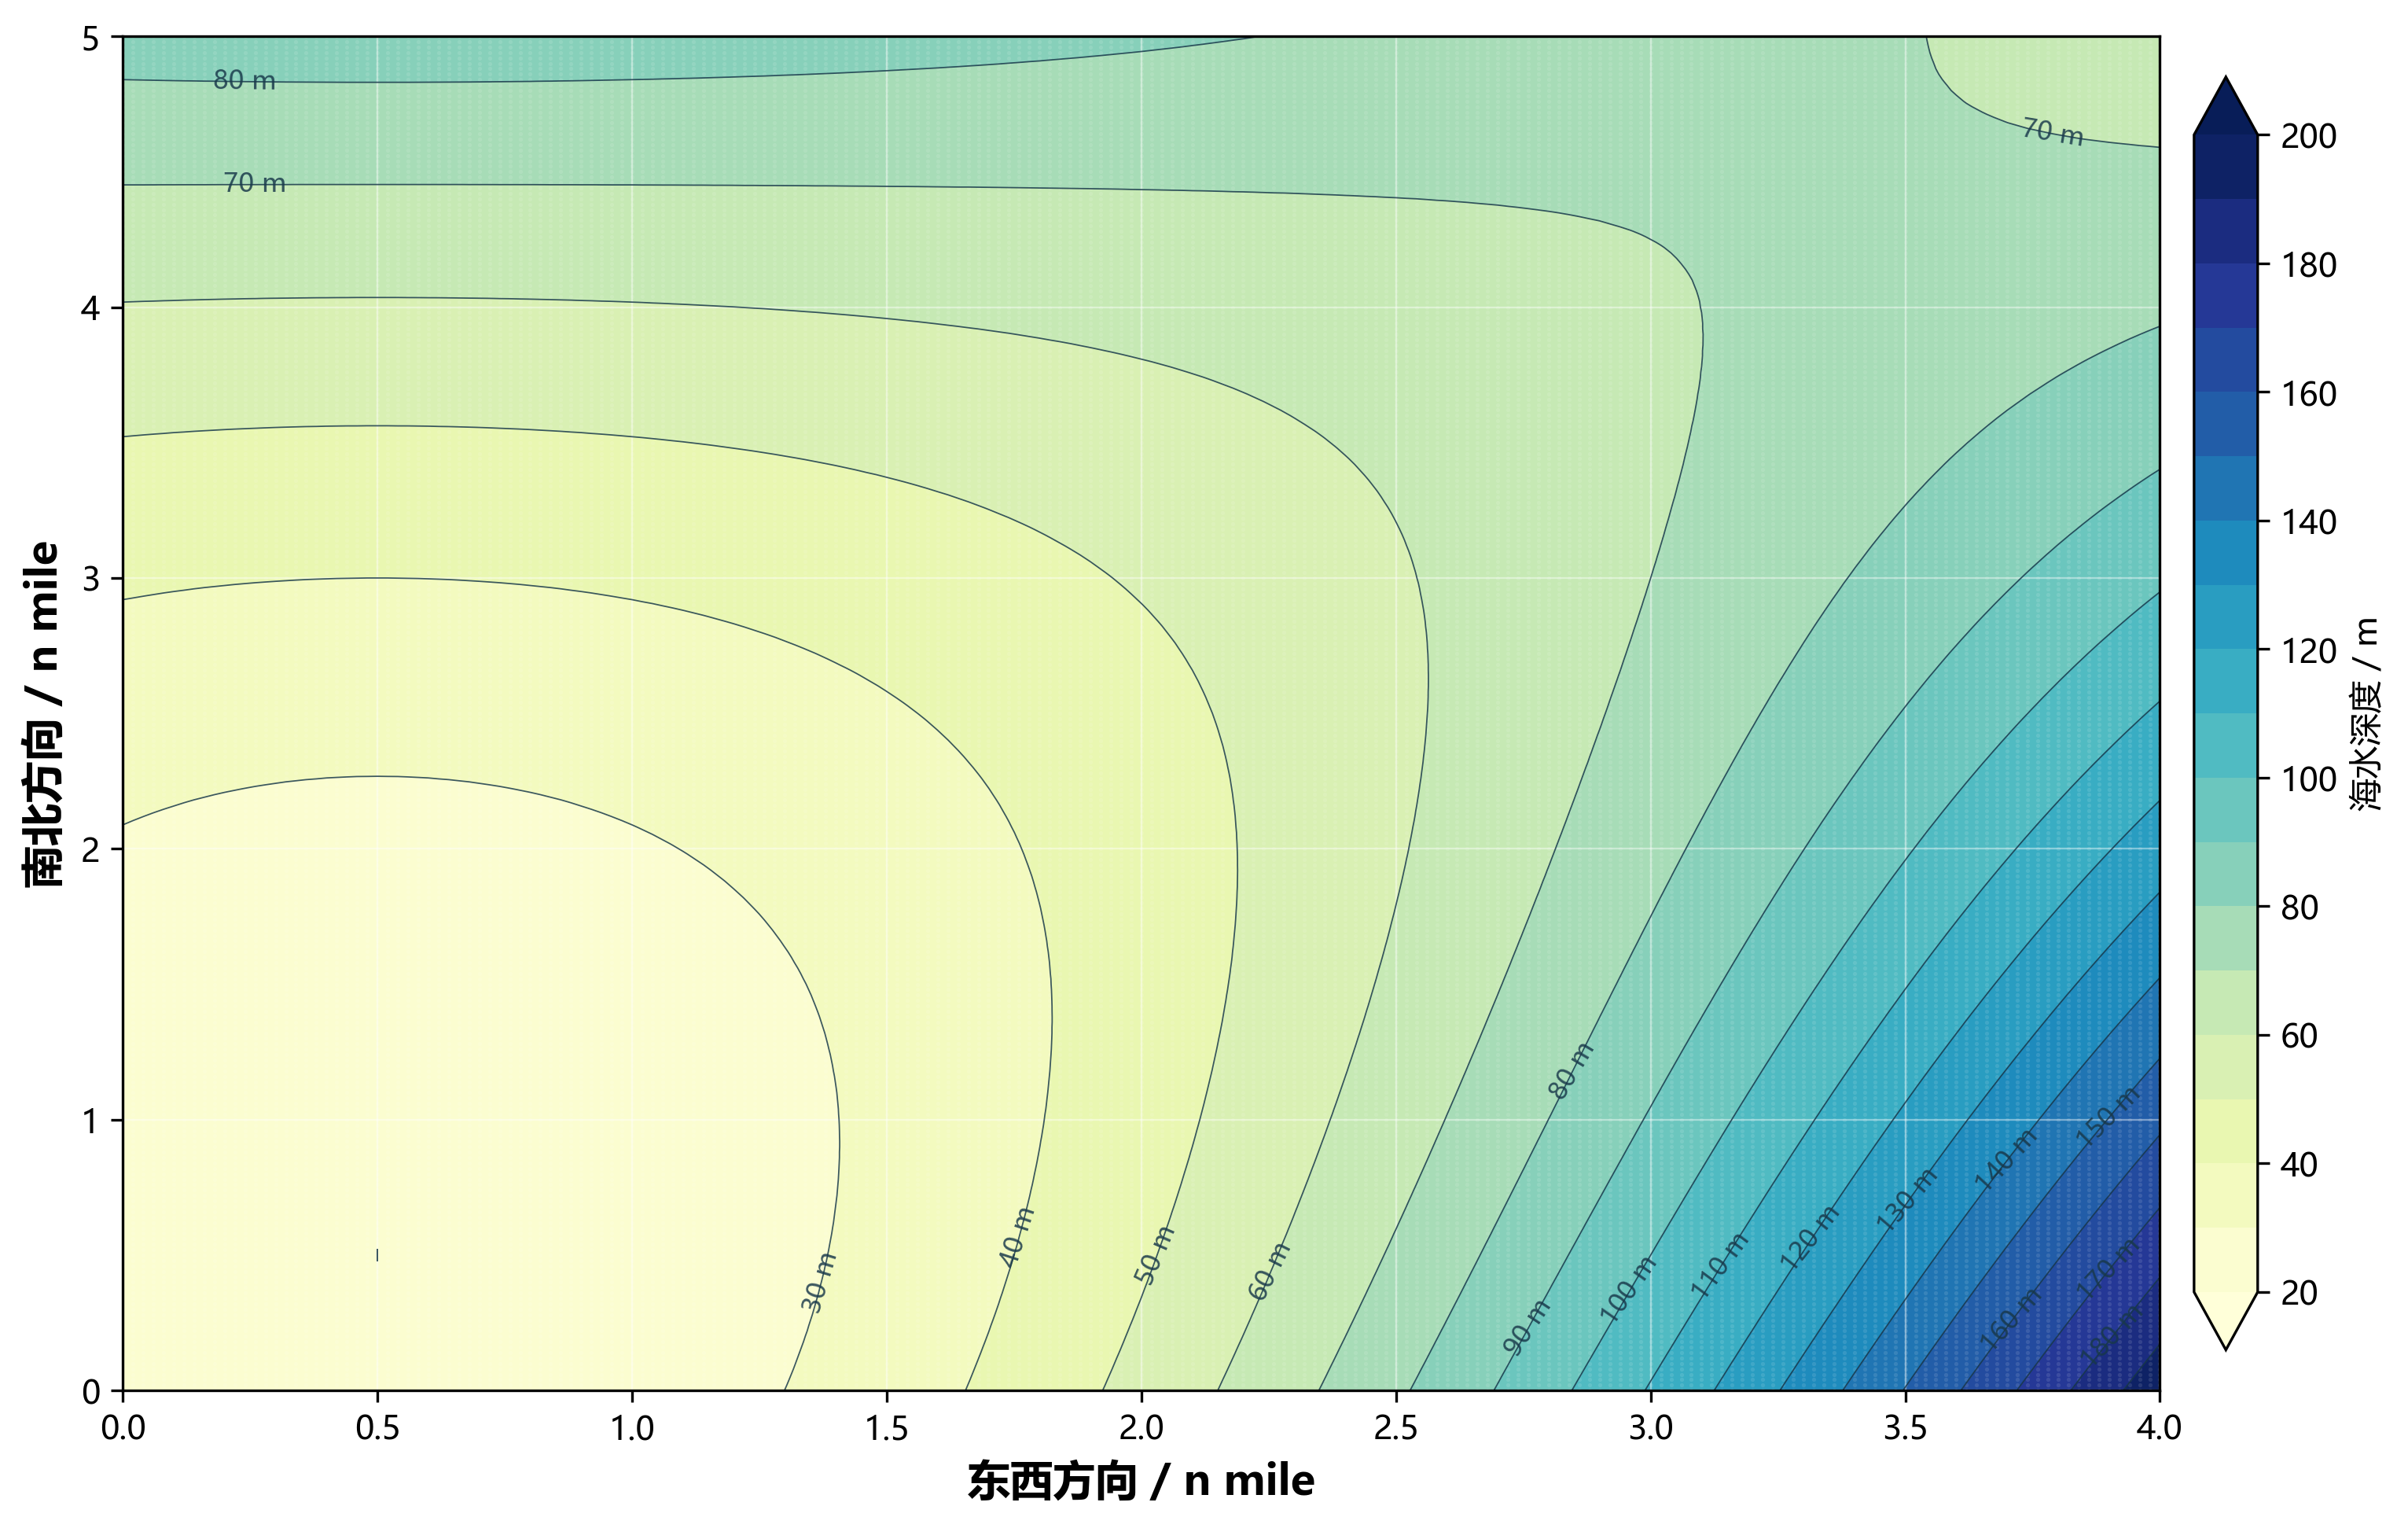
\includegraphics[width=.82\textwidth]{问题四/paper_q4_contour_revised_20260713.png}}
\\[0.8em]
\subcaptionbox{空间--水深 K-means 分区\label{fig:q4b}}{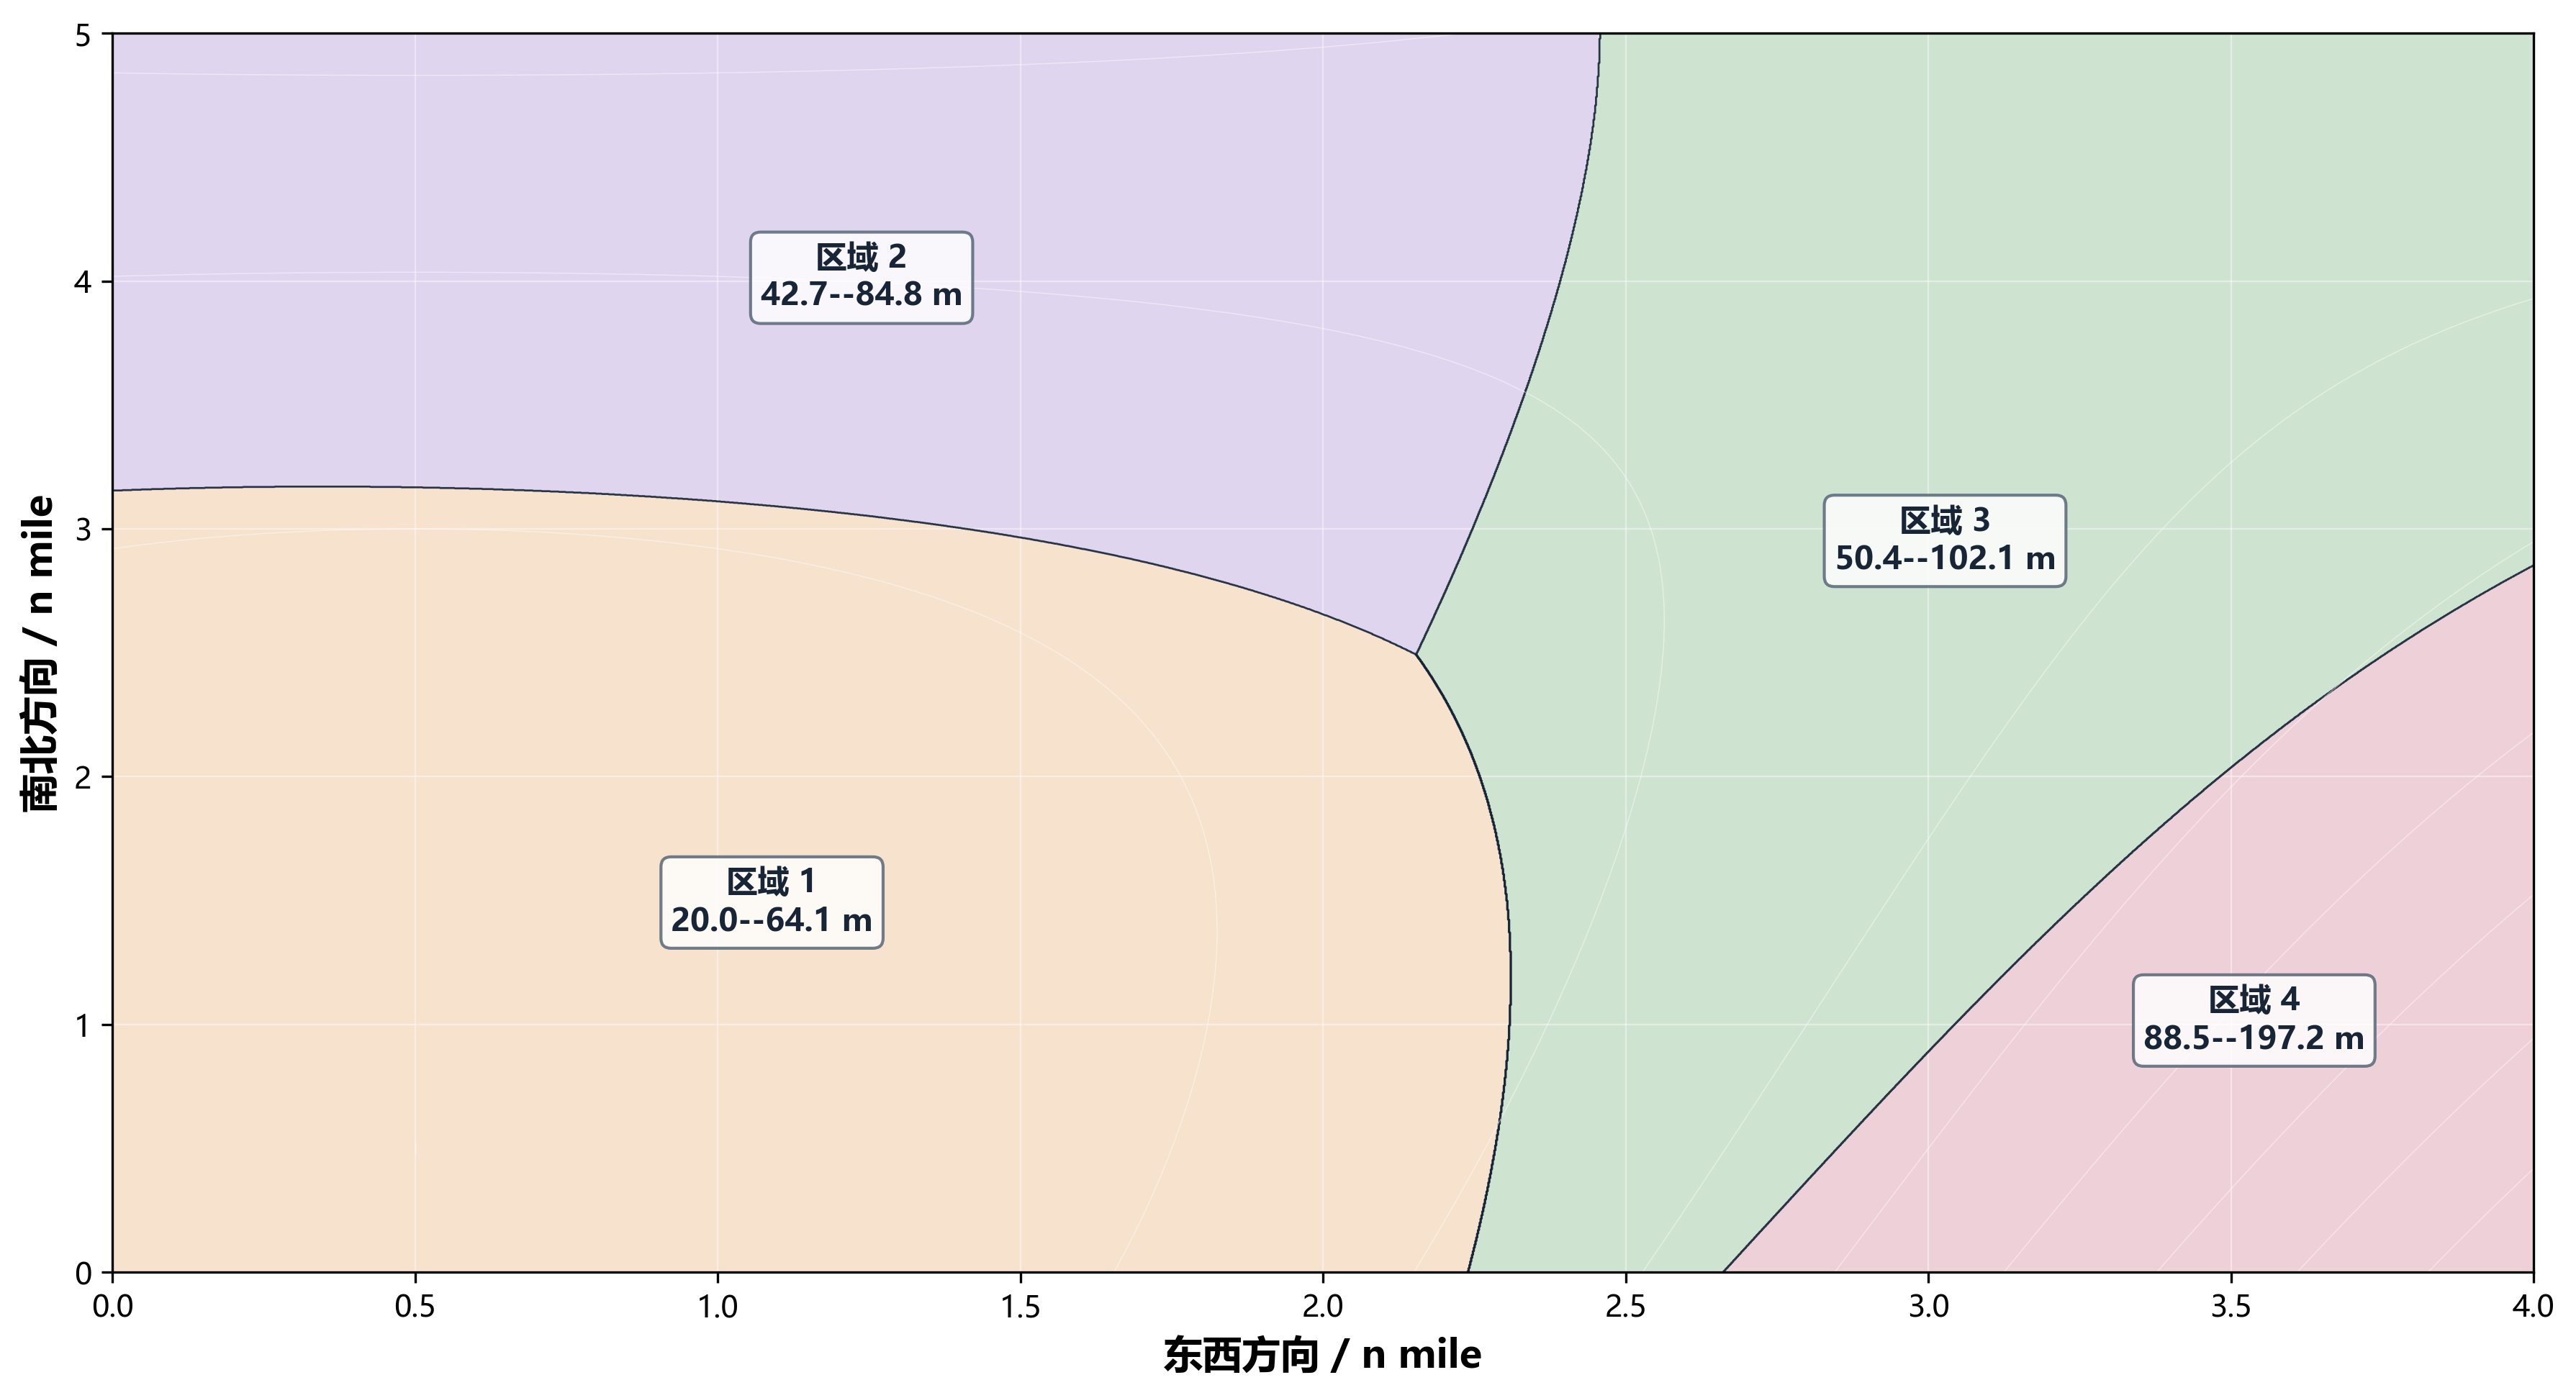
\includegraphics[width=.82\textwidth]{问题四/paper_q4_zones_revised_20260713.png}}
\caption{问题四地形重建与分区}
\label{fig:q4terrain}
\end{figure}

\subsection{沿等深线的曲线测线}
在第 $k$ 个分区内估计局部深度梯度 $g_k=\|\nabla D\|$。测线沿等深线布设，使其横向近似沿最大坡度方向。设曲线中心水深为 $h$，平底近似下半覆盖宽度为 $D\tan\gamma$；结合局部梯度修正后得到该测线覆盖的浅、深边界。相邻曲线的中心水深递推，使目标重叠率为 $\eta_k$。每条测线长度通过对应等深线在该分区内的折线段长度累加获得。

以四个分区的 $\boldsymbol\eta=(\eta_1,\ldots,\eta_4)$ 为决策变量，约束 $0.02\leq\eta_k\leq0.199$。理想情况下，令 $R_{\rm miss}$ 为未被任何条带覆盖的有效网格数占全部有效网格数的比例；令
$L_{>20\%}=\sum_j \ell_j\max(\eta_j-0.20,0)$ 为按相邻等深线长度加权的超额重叠等效长度。建立罚函数
\begin{equation}\label{eq:q4fitness}
F(\boldsymbol\eta)=L(\boldsymbol\eta)+1000L_{>20\%}(\boldsymbol\eta)+10^6R_{\rm miss}(\boldsymbol\eta).
\end{equation}
需要说明的是，当前程序通过各分区深度范围的首末边界递推生成测线，并将 $R_{\rm miss}=0$ 作为构造完成标志，尚未对二维空间网格重新计算独立的未覆盖面积。因此当前优化中该项不区分粒子，不能把输出的 0 直接等同于题目所要求的严格漏测面积比例；这也是本模型最需要补强的验证环节。
采用 28 个粒子、最多 12000 次迭代的粒子群算法求解，固定随机种子为 2023；连续 1000 次相对改进小于 $10^{-7}$ 后停止。最终在第 11000 次迭代满足停止条件。

\subsection{结果与指标}
优化得到
\begin{equation}
(\eta_1,\eta_2,\eta_3,\eta_4)=(0.020000,0.029569,0.020000,0.020000).
\end{equation}
最终 86 条曲线测线的评价指标见\cref{tab:q4result}。
\begin{table}[H]
\centering
\caption{问题四布线方案评价指标}
\label{tab:q4result}
\begin{tabularx}{0.82\textwidth}{LCR}
\toprule
指标 & 数值 & 单位\\
\midrule
测线数量 & 86 & 条\\
测线总长度 & 210.650322 & 海里\\
模型内漏测标志 & 0.000000 & --\\
超额重叠等效长度 & 0.000000 & 海里\\
\bottomrule
\end{tabularx}
\end{table}
表中 86 条测线及 $210.650322$ 海里总长度可由输出文件逐条累加复核；两个零值是当前深度带递推与目标重叠率上界下的模型内部指标。题目要求的漏测面积比例和重叠率超过 $20\%$ 部分的实际空间长度，仍需把每条曲线按局部覆盖宽度缓冲后，在二维网格上进行覆盖次数统计。故本文不把两个零值作为实际零漏测、零超额重叠的独立证据；在实际航测中还应为定位、姿态和声速误差保留安全裕度。

\cref{fig:q4layout}中蓝色区域为至少被一条测线覆盖的海域，橙色区域为相邻条带重叠部分，白色曲线为实际测线，橙色曲线强调重叠中心带。测线沿局部等深线弯曲，在西南浅水区较密，在东部深水区较疏，与覆盖宽度随水深增大的规律一致。优化在第 11000 次迭代达到稳定，四区目标重叠率分别为 $2.000\%$、$2.957\%$、$2.000\%$ 和 $2.000\%$；这些原先放在右侧摘要中的信息现统一移入正文，避免图片重复承载结论。

\begin{figure}[H]
\centering
\includegraphics[width=0.98\textwidth]{问题四/paper_q4_layout_revised_20260713.png}
\caption{问题四分区曲线测线布设结果}
\label{fig:q4layout}
\end{figure}

\section{模型检验与敏感性分析}
\subsection{特殊情形检验}
问题一在 $\alpha=0$ 时严格退化为平底覆盖宽度；问题二在 $\beta=0^\circ$ 时 $\alpha_\beta=0$，在 $\beta=90^\circ$ 时 $|\alpha_\beta|=\alpha$，均符合空间几何。问题三由角度搜索和改进粒子群两种独立方法得到同一最优方向和总长度，增强了数值结果可信度。

\subsection{参数敏感性}
由平底近似 $W=2D\tan(\theta/2)$ 可得
\[
\frac{\mathrm dW}{W}=\frac{\mathrm dD}{D}+\frac{\mathrm d\theta}{\sin\theta},
\]
其中 $\mathrm d\theta$ 以弧度计。因此水深相对误差按一比一传递到覆盖宽度；在 $\theta=120^\circ$ 附近，开角误差 $\pm1^\circ$ 对应覆盖宽度约 $\pm2.02\%$ 的相对变化。这一定量结果说明开角误差不能仅作次要扰动处理。目标重叠率增大将缩小相邻测线间距，从而增加测线数量和总长度；因此问题三在满足约束时取下限 $10\%$。问题四将目标重叠率下界设为 $2\%$ 是避免理论边界恰好相接的启发式选择，尚缺少不同下界下总长度与漏测风险的对比实验。

\subsection{误差来源}
主要误差来自：附件网格插值不能表达小尺度地形；局部坡度由有限差分估计；真实声线会因声速剖面弯曲；船舶定位和姿态改变实际条带边界；K-means 分区边界可能出现局部不连续。多波束系统能够高密度获取海底地形，但测量质量仍取决于声学环境、系统标定与数据处理\cite{hughesclarke}。实际应用应依据水道测量质量标准\cite{iho44}，通过加密测深点、加入安全重叠裕度及航后覆盖检查降低风险。

\section{模型评价与推广}
\subsection{优点}
\begin{enumerate}[label=\arabic*.]
  \item 从几何关系直接推导左右覆盖半宽，物理意义清晰，并统一了斜面距离与水平距离。
  \item 二维模型通过等效坡度自然推广到任意测线方向，特殊情形可验证。
  \item 理想海域采用可解释的角度搜索，真实海域采用分区曲线与粒子群，方法与地形复杂度匹配。
  \item 所有表格、测线坐标和评价指标均由程序输出，具有可复现性。
\end{enumerate}

\subsection{不足与推广}
\begin{enumerate}[label=\arabic*.]
  \item 问题四的漏测标志由深度带递推构造得到，尚未完成独立二维网格覆盖面积复核，也未包含设备和环境不确定性。
  \item 沿等深线布设会增加转向和曲线跟踪难度，未显式计入转弯半径与航行时间。
  \item 可进一步引入鲁棒优化，在随机水深误差和定位误差下最小化期望漏测；也可把测线长度、转弯代价与风险组成多目标优化，并生成 Pareto 前沿供实际作业选择。
\end{enumerate}

{\zihao{-5}
\begin{thebibliography}{9}
\bibitem{pso} Kennedy J, Eberhart R. Particle swarm optimization[C]//Proceedings of ICNN'95. IEEE, 1995: 1942--1948.
\bibitem{kmeans} MacQueen J. Some methods for classification and analysis of multivariate observations[C]//Proceedings of the Fifth Berkeley Symposium on Mathematical Statistics and Probability. 1967: 281--297.
\bibitem{lloyd} Lloyd S P. Least squares quantization in PCM[J]. IEEE Transactions on Information Theory, 1982, 28(2): 129--137.
\bibitem{lurton} Lurton X. An Introduction to Underwater Acoustics: Principles and Applications[M]. 2nd ed. Berlin: Springer, 2010.
\bibitem{hughesclarke} Hughes Clarke J E, Mayer L A, Wells D E. Shallow-water imaging multibeam sonars: a new tool for investigating seafloor processes in the coastal zone and on the continental shelf[J]. Marine Geophysical Researches, 1996, 18: 607--629.
\bibitem{iho44} International Hydrographic Organization. IHO Standards for Hydrographic Surveys, S-44[S]. Edition 6.2.0. Monaco: IHO, 2024.
\end{thebibliography}
}

\newpage
\begin{appendices}
\section{支撑材料列表}
\begin{table}[H]
\centering
\caption{主要支撑文件}
\begin{tabularx}{\textwidth}{LL}
\toprule
文件名 & 功能描述\\
\midrule
问题一/solve\_2023b\_q1.py & 问题一覆盖宽度、重叠率计算及绘图\\
问题一/result1.xlsx & 问题一表格结果\\
问题二/solve\_2023b\_q2.py & 问题二三维方向覆盖宽度计算\\
问题二/result2.xlsx & 问题二题目格式结果表\\
问题三/solve\_2023b\_q3\_angle\_search.py & 粗搜索与黄金分割优化\\
问题三/solve\_2023b\_q3\_pso.py & 改进粒子群复核程序\\
问题三/q3\_angle\_search\_lines.csv & 问题三最终测线坐标与属性\\
问题四/make\_contour\_from\_attachment.py & 附件读取、等深线提取与绘图\\
问题四/kmeans\_depth\_classification.py & 三维加权 K-means 分区\\
问题四/solve\_2023b\_q4\_kmeans\_curved\_lines.py & 分区曲线测线和粒子群优化\\
问题四/q4\_kmeans\_curved\_lines.csv & 问题四 86 条曲线测线数据\\
问题四/q4\_kmeans\_curved\_summary.csv & 问题四最终评价指标\\
\bottomrule
\end{tabularx}
\end{table}

\section{主要算法流程}
\begin{enumerate}
  \item 读取题设参数或附件测深矩阵，统一海里与米的单位；
  \item 依据\cref{eq:depth1,eq:ws,eq:wh}计算局部水深和覆盖宽度；
  \item 问题三遍历方向角，递推满足重叠约束的测线截距，再以黄金分割精修；
  \item 问题四对标准化空间--水深特征聚类，提取各区等深线长度查找表；
  \item 粒子群优化各分区目标重叠率，以\cref{eq:q4fitness}评价粒子；
  \item 输出测线坐标、总长度、模型内漏测标志、超额重叠等效长度及布线图。
\end{enumerate}

\section{核心代码功能片段}
本附录仅列出与论文公式和求解流程直接对应的核心函数；完整程序及输出文件见附录 A。代码片段直接读取项目脚本，避免论文代码与实际实现不一致。

\subsection{问题一：水深、覆盖半宽与重叠率}
以下函数分别实现式\cref{eq:depth1,eq:ws,eq:eta}所对应的水深、左右覆盖半宽及相邻条带重叠率计算。
\lstinputlisting[firstline=22,lastline=35,firstnumber=22,caption={问题一水深与覆盖宽度核心函数}]{问题一/solve_2023b_q1.py}
\lstinputlisting[firstline=54,lastline=65,firstnumber=54,caption={问题一重叠率批量计算}]{问题一/solve_2023b_q1.py}

\subsection{问题二：任意方向等效坡度}
该函数先把角度由度转换为弧度，再计算等效坡度、船位水深及斜面和水平投影覆盖宽度。
\lstinputlisting[firstline=29,lastline=48,firstnumber=29,caption={问题二任意方向覆盖宽度计算}]{问题二/solve_2023b_q2.py}

\subsection{问题三：粒子适应度与约束罚项}
该函数对应公式（15），同时检查深浅水边界覆盖和相邻条带 $10\%\sim20\%$ 的重叠约束。
\lstinputlisting[firstline=305,lastline=330,firstnumber=305,caption={问题三粒子群适应度函数}]{问题三/solve_2023b_q3_pso.py}

\subsection{问题四：空间--水深特征与 K-means 更新}
代码对东西坐标、南北坐标和水深进行标准化加权，并执行簇分配与中心更新；这与正文中的特征向量和聚类目标一致。
\lstinputlisting[firstline=165,lastline=194,firstnumber=165,caption={问题四加权 K-means 核心计算}]{问题四/kmeans_depth_classification.py}
\end{appendices}

\end{document}
